\documentclass[a4paper,10pt]{article}
\usepackage[utf8]{inputenc}
\usepackage[UKenglish]{babel}
\usepackage{fancyhdr}
\usepackage{anysize}
\usepackage{amsmath, amsthm, amssymb}
\usepackage{lastpage}
\usepackage[all]{xy}  % drawings
%\usepackage{listings} % code highlighting
\usepackage[usenames,dvipsnames]{color}
\usepackage{graphicx}
\usepackage{caption}
\usepackage{subfigure}

\pagestyle{fancy}
\fancyfoot[R]{\em \thepage / \pageref{LastPage}}
\fancyfoot[C]{}
\fancyfoot[L]{\em Master VIBOT}
\fancyhead[R]{\em Lab3 - Particle Filter}
\fancyhead[C]{}
\fancyhead[L]{\em Probabilistic Robotics}
\renewcommand{\headrulewidth}{0.4pt}
\renewcommand{\footrulewidth}{0.4pt}

%\,	 a small space
%\:	 a medium space
%\;	 a large space
%\quad	 a really large space
%\qquad	 a huge space
%\!	 a negative space (moves things back to the left)
        
\begin{document}

\marginsize{2cm}{2cm}{2cm}{2cm}

% Title
%\hspace{1mm}
\begin{center}
\Large \textbf{Lab3 - Particle Filter}
\end{center}
%\hspace{1mm}

%===============================================================================
\section{Introduction}

This lab is designed to implement a Particle Filter or Montecarlo Localization (MCL) algorithm to localize a two dimensional robot (turtlebot) in a given map. The bagfile provided is the same as in the previous lab.

\subsection{Particle Filter}

The MCL localization is an implementation of the Markovian localization problem where the involved pdfs are represented through samples (particles) and the Bayes filter is implemented through the Particle Filter. Markov localization addresses the problem of state estimation from sensor data. Markov localization is a probabilistic algorithm: Instead of maintaining a single hypothesis as to where in the world a robot might be, Markov localization maintains a probability distribution over the space of all such hypotheses. The probabilistic representation allows it to weigh these different hypotheses in a mathematically sound way.

%===============================================================================
\section{Pre-lab}

Review the particle filter explained on lectures and write the prediction step in Python code, given the particles position in $(x,y)$ as a numpy array named \texttt{p\_xy} of shape $2 \times N$ and their orientations being an array named \texttt{p\_ang} of dimension $N$.

%===============================================================================
\section{Lab work}

The folder named \texttt{lab3\_particlefilter} contains the code for running this lab. Your solution of the previous lab \texttt{lab2\_splitandmerge} will be called to provide the lines input for the particle filter localization. You can test the code by running:

\begin{verbatim}
    roslaunch lab3_particlefilter particle_filter.launch
\end{verbatim}

As you can see the dummy Particle Filter algorithm implemented, only initializes the particles along the extension of the map, nothing else. The three parts of the filter that must be implemented are:

\begin{description}
    \item[Prediction] Compute the new position $(x, y, \theta)$ of the particles given an odometry measurement $(\Delta x, \Delta y, \Delta \theta )$ in the vehicle frame. Do not forget to add the odometry Gaussian noise in the increments.
    
    \item[Weighting] Compute the weight of each particle by comparing the lines obtained from the measurements with the lines of the given map. To be compared, the lines have to be transformed from the form [x1 y1 x2 y2] to the representation [range angle] defined by the shortest distance from the origin to the line (perpendicular distance) being the range, and the angle of this range seen from the origin (Fig.~\ref{repr}).
    
    \begin{center}
        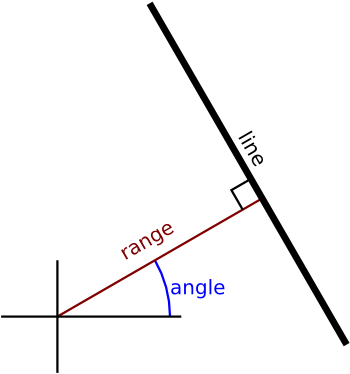
\includegraphics[width=0.25\textwidth]{pict/lab3-repr}
        \captionof{figure}{Representation of a line in (range, angle).}
        \label{repr}
    \end{center}
    
    The comparison must be computed with a Gaussian as
    \begin{equation}
        w = \frac{1}{\sigma \sqrt{2 \pi}} \exp \left[ - \frac{(x - \mu)^2}{2 \sigma^2} \right]
    \end{equation}
    being $x$ the measured value (range or angle), $\mu$ the expected value (extracted from given map lines) and $\sigma$ the uncertainty of the measurement. Since range and angle uncertainties are independent they can be multiplied to obtain the final weight.
    
    Lines measured can be compared to all lines in the map and take the best results or associating them by searching the most likely one and then computing the weight. Remember that map lines are represented on the world frame and the measured lines in the robot frame (each particle own frame).
    
    \item[Resampling] Systematic resampling, as explained in lectures, will be used in this lab.
\end{description}

%===============================================================================
\section{Optional}

Improve the localization by taking into account if the segments extracted from the measurements coincide with the segments in the given map. Not only compare the representation in range and angle (Fig.~\ref{optional}). This will discern more properly which measurements can be associated with which map features.

\begin{center}
	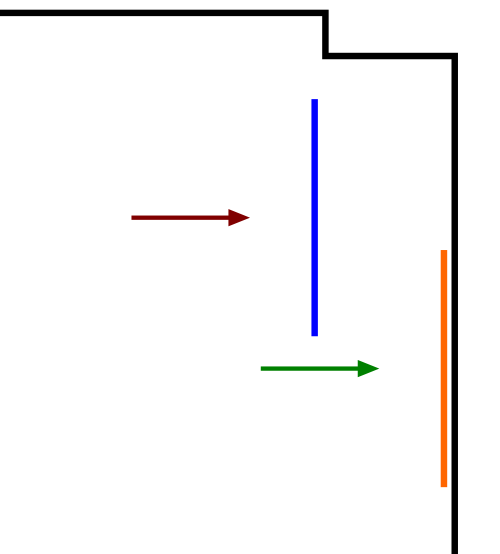
\includegraphics[width=0.40\textwidth]{pict/lab3-optional}
	\captionof{figure}{If only range and angle representation of lines is used for weighting, both red and green particles have the same weight because they coincide with lines at same angle and distance (red with the small line on top). If segments are checked, the blue measurement of the red particle cannot belong to the small line on top and its weight will be smaller than the green particle whose orange measurement agrees completelly with the given map.}
	\label{optional}
\end{center}

%===============================================================================
\section{Lab report}

Write a brief report (maximum 2 pages) explaining your solution and problems faced. Include the final code in the zip file (not in the report).

\end{document}
